\chapter{NOVEL METHOD USING ANATOMICAL PRIOR INFORMATION}
\label{ch:new_model}
%


When considering using more than one data modality for analysis, there are many ways to combine them. 
%
The asymmetric multi-modal data analysis paradigm consists of selecting a tool designed for one data modality and incorporating information from all the other data modalities into the analysis.
%
This paradigm fits the purpose of performing the Electronic Source Imaging while incorporating information from additional data modalities.

%Within the asymmetric multi-modal data analysis paradigm, we aim to enhance the ESI data by incorporating information from other measurement modalities.

In particular, we consider the case in which a physical region is known to produce a higher background electrical activity.
%
The location and extent of this region are observed using some imaging techniques independent of EEG.

The motivation for this particular setup comes from a specific experimental setup in which an ischemic stroke is induced, and later, the affected area is determined using histochemical analysis.

\section{Model Assumptions}

The relationship between the recordings from surface electrodes, $\Y$, and the magnitudes of equivalent distributed dipoles located inside the brain, $\SA$, is given by the following equation
\begin{equation}
\Y = \G \ppar{\SA + \varepsilon},
\label{eq:3.1}
\end{equation}
with $\Y \in \R^{M \times 1}$, $\SA \in \R^{3N \times 1}$, $\G \in \R^{3N\times M}$, and $\varepsilon\in \R^{N\times 1}$.
%
This model was described in detail in Chapter \ref{ch:forward}, including the interpretation and derivation of the leadfield matrix $\G$.
%
Notice that this model considers only internal noise.

Ideally, the extra information provided by the additional data modality should allow us to identify an anatomical region exhibiting pathological behavior; for simplicity, we refer to this region as a P-region. 
%
For generality, we consider the possibility of multiple disjoint P-regions, say $K$ with $1\leq K < \infty$.
%
P-regions are labeled $P_1, P_2, \dots, P_K$, with $P_0$ the dipoles outside all P-regions.
%
For notation, define 
\begin{equation}
    P_k = \sset{ n\in \sset{1, 2, \dots, N} \given n\text{-th dipole is in the } k\text{-th region} }
\end{equation}

\begin{figure}
    \centering 
    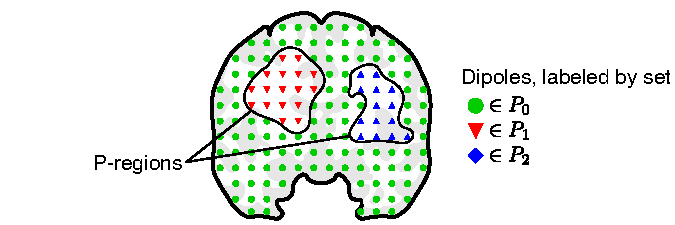
\includegraphics{./img/Pregions_pic.pdf}
    \caption{Construction of labels based on P-regions, representing regions when a particular symptom, independent of electrophysiological measurements, was observed.}
\end{figure}

As a remark, the P-regions are defined independently of the dipoles; each $P_k$ is the set of dipoles inside a specific P-region.
%
If a different set of dipoles is selected for the same subject and pathology data, the P-regions will change but will be constructed in the same anatomical space.

For ease of handling in the model, the P-regions regions are encoded using the matrix 
$\PA\in \sset{0,1}^{N\times K}$ defined as
\begin{equation}
    \PA\ppar{n,k} = \begin{cases}
        1, &\text{if } n \in P_k \\
        0, &\text{otherwise.}
    \end{cases}
\end{equation}

%In section \ref{sec:SelectPregions}, we describe heuristic methods to determine the P-regions and, consequently, the matrix $\PA$.

%\begin{figure}
%\centering
%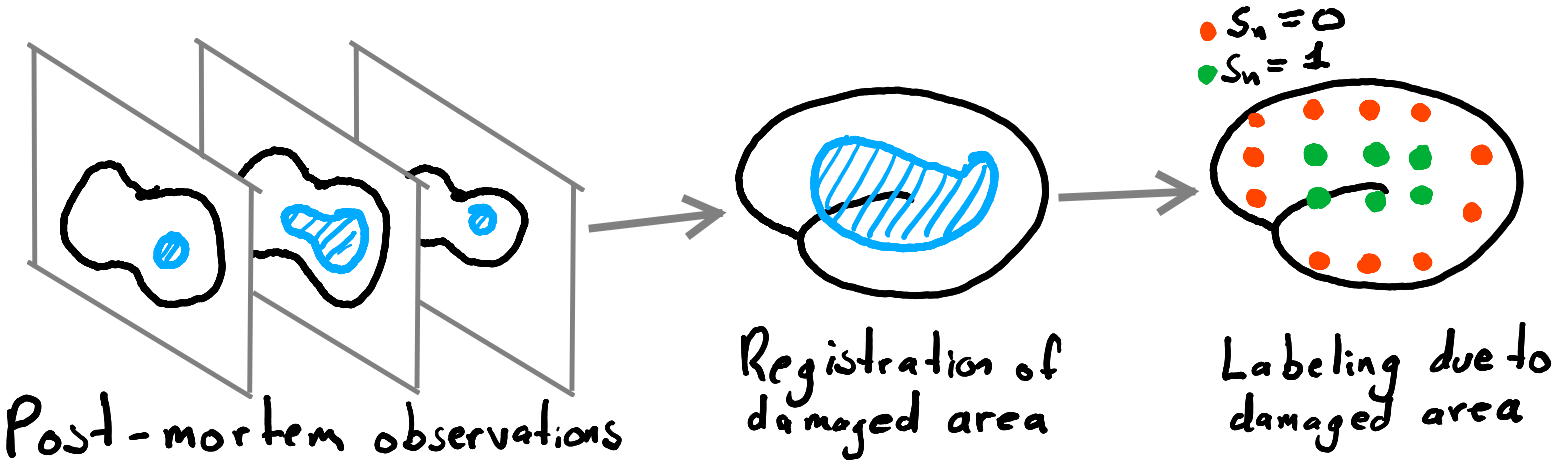
\includegraphics[width=0.8\linewidth]{./img/sketch02_v2}
%\end{figure}

The relation between the current density, $\SA$, and the P-regions is incorporated into the model by adjusting the covariance of $\SA$ depending on which P-region it is located.
%
To be specific, consider,
\begin{equation}
    \ccov{\SA\ppar{n_1}, \SA\ppar{n_2}} = 
    \begin{cases}
        \gamma_k, & \text{if } n_1, n_2\in P_k, \\
        0, & \text{otherwise}
    \end{cases}
\end{equation}
with $0 < \gamma_0 \ll \gamma_k$ for $1\leq k \leq K$.
%
This guarantees that P-regions have synchronized activity that is larger in magnitude than the background activity.

The assumption of a perfect synchrony is introduced in order to simplify the model.
%
We can separate the source, $\SA$, into a regionally-synchronized activity, $\RA$, and a background noise, $\BA$, as
\begin{equation}
    \SA +\varepsilon = \BA + \PA \RA = \BA + \sum_{k=1}^K \PA(:,k)\, \RA(k)
    \label{eq:3.4}
\end{equation}
with $\BA \in \R^{N\times 1}, \RA \in \R^{K\times 1}$ independent with each other.
%
These assumptions about P-regions can be combined with Gaussian assumptions, leading to 
\begin{align}
    \BA &\sim \norm\ppar{0, \gamma_0 \id_N } 
    \label{eq:3.5} \\
    \RA &\sim \norm\ppar{0, 
    \spar{\text{diag}\ppar{\gamma_1, \gamma_2, \dots, \gamma_K}-\gamma_0 \id_K} }
    \label{eq:3.6}
\end{align}

%%%%%%%%%%%%%%%%%%%%%%%%%%%%%%%%%%%%%%%%%%%%%%%%%%%%%%%%%%%%%%%%%%%%%%%%

\section{Proposed Estimator}

Given the assumptions described in the previous section, we propose constructing a linear estimator for $S$ similar to those presented in Chapter \ref{ch:review}.
%
%This choice follows the analysis of strengths and weaknesses. 
%
This choice follows the expectation of short computation times and memory requirements. 
%
We expect that the additional information from P-regions will decrease spatial dispersion while not significantly increasing computational speed.


The estimator of $\SA$ will be constructed as a Maximum A Posteriori estimator, maximizing the log probability of $\left. \SA \given \Y \right.$, as
\begin{align}
    \hat{\SA} &= 
    \argmax_{\SA }\, 
    \phantom{.}
    \log\ppar{
    \text{Prob}\ppar{ \SA \given \Y }}
    \nonumber \\
    &=
    \argmax_{\SA }\, 
    \phantom{.}
    \log \ppar{
    \text{Prob}\ppar{ \Y \given \SA }\,  \text{Prob}\ppar{ \SA } }
\end{align}
the structure of P-regions is incorporated by using the following decomposition
\begin{equation}
    {\SA} = {\BA} + \PA {\RA}
    = {\BA} + \sum_{k=1}^K \PA(:,k) {\RA}(k)
    \label{eq:3.7_v2}
\end{equation}
and the model equation $\Y = \G \SA$ is incorporated as a constraint, resulting in the following optimization problem
\begin{align}
    \sset{ \hat{\BA}, \hat{\RA} } 
    =
    \argmax_{\BA, \RA }\, 
    &\phantom{.}
    \frac{\sigma}{2 \gamma_0} \nnorm{\BA}^2
    +
    \sum_{k=1}^K \frac{\sigma}{2\ppar{\gamma_0-\gamma_k} } \nnorm{\PA(:,k)\, \RA(k)}^2
    \nonumber \\
    \text{s.t.}
    \quad
    &\phantom{.}
    {\G \ppar{\BA + \PA \RA} } - \Y = 0
    \label{eq:3.7}
\end{align}
where $\gamma_0, \gamma_1, \dots, \gamma_k, \sigma \in \R_+$ are parameters related to the assumed distributions of $\BA$ and $\SA$ given in equations \eqref{eq:3.5} and \eqref{eq:3.6}.
%
For ease of notation, we define the following equivalent parameters
\begin{align}
    \theta_0 &= \frac{1}{\sigma} \gamma_0 \\
    \theta_k &= \frac{1}{\sigma} \ppar{ \gamma_k- \gamma_0 },
    \text{ for } k = 1, 2, \dots, K.
\end{align}

Notice that the parameter $\sigma$ scales all the other parameters $\gamma_k$ equally, and thus, it can be ignored when discussing their relative magnitudes only.

%A careful derivation will reveal that $\theta_0 = \frac{\gamma_0 }{\sigma}$ and $\theta_k = \frac{\gamma_k-\gamma_0}{\sigma}$, with $\sigma>0$ the variance of the external noise.
%
%However, we decided that the role of those parameters within the interpretability of the model is negligible; we use $\theta_k$ as generic parameters that need to be tuned using the heuristics discussed in Chapter 2.

The constrained optimization problem in equation \eqref{eq:3.7} is solved using the method Lagrange multipliers.
%
First, we construct the respective Lagrangian function
\begin{align}
    \mathcal{L}\ppar{\BA, \RA, \lambda} &=
    \frac{1}{2 \theta_0} \nnorm{\BA}^2
    +
    \sum_{k=1}^K \frac{1}{2 \theta_k} \nnorm{\PA(:,k)\, \RA(k)}^2
    +
    \lambda^T \ppar{{\G \ppar{\BA + \PA \RA} } - \Y}
\end{align}
which can be minimized by solving the normal equations, i.e., the partial derivatives equal to zero.
%
The partial derivatives are given by
\begin{align}
    \frac{\partial}{\partial \BA} \mathcal{L}\ppar{\BA, \RA, \lambda}
    &=
    \frac{1}{\theta_0} \BA + \G^T \lambda 
    \label{eq:3.9}
    \\
    \frac{\partial}{\partial \RA(k)} \mathcal{L}\ppar{\BA, \RA, \lambda}
    &=
    \frac{1}{\theta_k} \PA(:,k)^T \PA(:,k)\, \RA(k) + \PA(:,k)^T \G^T \lambda 
    \label{eq:3.10}
    \\
    \frac{\partial}{\partial \lambda} \mathcal{L}\ppar{\BA, \RA, \lambda}
    &=
    \G \ppar{ \BA + \PA \RA } - \Y
    \label{eq:3.11}
\end{align}

Solving the normal equation for \eqref{eq:3.9} and \eqref{eq:3.10} lead to the following identities
\begin{align}
    \BA &= -\theta_0 \G^T \lambda
    \label{eq:3.13}
    \\
    \RA(k)
    &=
    -\theta_k \spar{\PA(:,k)^T \PA(:,k)}^{-1} \PA(:,k)^T \G^T \lambda 
    \label{eq:3.14}
\end{align}

Notice that $\PA(:,k)^T \PA(:,k) \in \mathbb{N}^{1\times 1}$ represents the number of dipoles on the $k$-th P-region, and thus is invertible.
%
For ease of notation, define
\begin{equation}
    \abss{P_k} = \PA(:,k)^T \PA(:,k)
\end{equation}

From equation \eqref{eq:3.11}, we may obtain a closed-form expression for $\lambda$,
\begin{align}
    \Y
    &=
    \G \BA + \G { \sum_{k=1}^K { \PA(:,k)\, \RA(k) } }
    \nonumber \\
    &=
    \G\ppar{-\theta_0 \G^T \lambda}
    + \G \sum_{k=1}^K
    { \PA(:,k)\, \ppar{-\theta_k \abss{P_k}^{-1} \PA(:,k)^T \G^T \lambda}}
    \nonumber \\
    &=
    -\G \ppar{ \theta_0 \id_N + \sum_{k=1}^K \theta_k \abss{P_k}^{-1} 
    \PA(:,k)\, \PA(:,k)^T
    } \G^T \lambda
\end{align}
which leads to the following identity
\begin{equation}
    \lambda
    =
    -\spar{\G \ppar{ \theta_0 \id_N + \sum_{k=1}^K \theta_k \abss{P_k}^{-1} 
    \PA(:,k)\, \PA(:,k)^T
    } \G^T}^{-1} \Y
\end{equation}

For robustness and to ensure that the resulting matrices are invertible, we propose using a regularized $\lambda_\rho$, defined as
%\begin{equation}
%    \lambda_\rho
%    =
%    -\spar{\G \ppar{ \theta_0 \id_N + \sum_{k=1}^K \theta_k \abss{P_k}^{-1} 
%    \PA(:,k)\, \PA(:,k)^T
%    } \G^T + \rho \id_M }^{-1} \Y
%\end{equation}
%and for a further simplification of notation, define
\begin{align}
    \lambda_\rho &= -W_\rho  \Y 
    \\
    W_\rho &=
    \spar{\G \ppar{ \theta_0 \id_N + \sum_{k=1}^K \theta_k \abss{P_k}^{-1} 
    \PA(:,k)\, \PA(:,k)^T
    } \G^T + \rho \id_M }^{-1}
\end{align}
where $\rho>0$ is a regularization parameter that must be determined using any of the heuristics defined in Chapter \ref{ch:review}.

Using $\lambda_\rho$ in equations \eqref{eq:3.13} and \eqref{eq:3.14} lead to the estimators
\begin{align}
    \hat{\BA} &=
    \theta_0 \G^T W_\rho \Y
    \\
    \hat{\RA}(k) &=
    \theta_k \abss{P_k}^{-1} \PA(:,k)^T \G^T W_\rho \Y
\end{align}

The estimator for $\SA$ is constructed as in equation \eqref{eq:3.7_v2},
\begin{align}
    \hat{\SA}
    &=
    \hat{\BA} + \sum_{k=1}^K \PA(:,k) \hat{\RA}(k)
    \nonumber \\
    &=
    \ppar{\theta_0 \G^T W_\rho \Y}
    + \sum_{k=1}^K \PA(:,k) \ppar{\theta_k \abss{P_k}^{-1} \PA(:,k)^T \G^T W_\rho \Y}
    \nonumber \\
    &=
    \ppar{ \theta_0 \id_N + \sum_{k=1}^K \theta_k \abss{P_k}^{-1} 
    \PA(:,k)\, \PA(:,k)^T
    } \G^T W_\rho \Y
\end{align}

Thus, the proposed estimator is given by
\begin{align}
    \hat{\SA}
    &=
    \ppar{ \theta_0 \id_N + \sum_{k=1}^K \theta_k \abss{P_k}^{-1} 
    \PA(:,k)\, \PA(:,k)^T
    } \G^T W_\rho \Y
    %\label{eq:3.24}
    \\
    W_\rho &=
    \spar{\G \ppar{ \theta_0 \id_N + \sum_{k=1}^K \theta_k \abss{P_k}^{-1} 
    \PA(:,k)\, \PA(:,k)^T
    } \G^T + \rho \id_M }^{-1}
    %\label{eq:3.25}
\end{align}

For ease of notation, the parameter $\theta_0$ will be replaced by rewriting
\begin{align}
    \hat{\SA}
    &=
    \ppar{ \id_N + \sum_{k=1}^K \tau_k \abss{P_k}^{-1} 
    \PA(:,k)\, \PA(:,k)^T
    } \G^T W_\lambda \Y
    \label{eq:3.24}
    \\
    W_\lambda &=
    \spar{\G \ppar{ \id_N + \sum_{k=1}^K \tau_k \abss{P_k}^{-1} 
    \PA(:,k)\, \PA(:,k)^T
    } \G^T + \lambda \id_M }^{-1}
    \label{eq:3.25}
\end{align}
with $\tau_k = \theta_k/\theta_0 > 1$ and $\lambda=\rho/\theta_0$.

\subsection{Implementation notes}

The computation of the estimator described in equations \eqref{eq:3.24} and \eqref{eq:3.25} can be accelerated by avoiding explicit matrix multiplications whenever possible.
%
For instance, consider the matrices in the form 
\begin{equation}
    A_k = \abss{P_k}^{-1} \PA(:,k)\, \PA(:,k)^T
\end{equation}
for $1\leq k \leq K$. 
%
Notice that each $A_k \in \R^{N\times N}$ is an averaging operator with support over the corresponding P-region.
%
In other words, for any vector $V\in \R^{N}$ we have
\begin{equation}
    \spar{A_k V}(n) =
    \begin{cases}
        {\displaystyle \frac{1}{\abss{P_k}} \sum_{n'\in P_k} V(n')}, 
        &\text{if } n\in P_k, \\
        0, &\text{otherwise}.
    \end{cases}
    \label{eq:4.30}
\end{equation}

With this notation at hand, we can rewrite equation \eqref{eq:3.24} as
\begin{align}
    \hat{\SA}
    &=
    \ppar{\id_N + \sum_{k=1}^K \tau_k A_k}\G^T W_\lambda \Y
\end{align}

%Instead of constructing the matrix $\ppar{\theta_0 \id_N + \sum_{k=1}^K \theta_k A_k}$ explicitly 

Using the matrices $A_k$, we can construct $\hat{\SA}$ row-by-row as follows:
\begin{align}
    \hat{\BA}_0
    &=
    \G^T W_\lambda \Y \\
    \hat{\RA}_0(k)
    &=
    {\displaystyle \frac{1}{\abss{P_k}} \sum_{n\in P_k} \hat{\BA}_0(n)},
    \text{for } 1\leq k \leq K
    \\
    \hat{\SA}
    &=
    \hat{\BA}_0 + 
    \sum_{k=1}^K
    \tau_k \G\, \hat{\RA}_0(k)
    \label{eq:3.s1}
\end{align}
with $\hat{\BA}_0 \in \R^{N\times 1}$, $\hat{\RA}_0 \in \R^{K\times 1}$.
%
Alternatively, we can construct $\hat{\SA}$ row by row as
\begin{equation}
    \hat{\SA}(n) =
    \begin{cases}
        \hat{\BA}_0(n) + \tau_k \hat{\RA}_0(k),
        &\text{if } n\in P_k \text{ with } 1\leq k \leq K,
        \\
        \hat{\BA}_0(n), &\text{if } n\in P_0
    \end{cases}
    \label{eq:3.s2}
\end{equation}
Depending on how large the P-regions are, i.e., how large are each $\abss{P_k}$ with respect to $N$, it would be more convenient to use
either \eqref{eq:3.s1} or \eqref{eq:3.s2}.
%
In a practical setting, we informally expect each P-region to contain less than 10\% of the total dipoles.

%%%

Next, equation \eqref{eq:3.25} is simplified by considering the properties of the matrices involved.
%
Notice that each matrix $A_k$ is symmetric and idempotent.
%
Furthermore, if the P-regions are non-intersecting, then
\begin{equation}
    A_{k_1} A_{k_2} = 
    \begin{cases}
        A_{k_1}, &\text{if } k_1=k_2, \\
        0, &\text{otherwise.}
    \end{cases}
    \label{eq:3.27}
\end{equation}

This property can be extended to get powers and decomposition of the averaging operators $A_k$.
%
In particular, we have the following
\begin{equation}
    \spar{q_0 \id_N + \sum_{k=1}^K q_k A_k}^2
    =
    q_0^2 \id_N + \sum_{k=1}^K \ppar{2q_0 q_k + q_k^2} A_k
\end{equation}
which leads to the following identity
\begin{equation}
    \spar{\id_N + \sum_{k=1}^K \ppar{\sqrt{1+\tau_k}-1} A_k}^2
    =
    \id_N + \sum_{k=1}^K {\tau_k} A_k
\end{equation}

For ease of notation, define
\begin{align}
    \AAA_{\Theta} &=
    \id_N + \sum_{k=1}^K \ppar{\sqrt{1+\tau_k}-1} A_k
\end{align}

With this decomposition at hand, we can rewrite $W_\lambda$ as
\begin{equation}
    W_\lambda =
    \spar{ \ppar{\G \AAA_{{\Theta}}} \ppar{\G \AAA_{{\Theta}}}^T
    + \rho \id_M }^{-1}
\end{equation}

Notice that $\AAA_\Theta\in \R^{N\times N}$ is a sum of matrices in the form of $A_k$ which, as seen in equation \eqref{eq:4.30}, 
work as averaging operators.
%
We can conclude that $\AAA_\Theta$ acts as a weighted average operator over the rows of $\G$. In other words, we can write
\begin{equation}
    \spar{\G \AAA_\Theta}(:, n) =
    \begin{cases}
    \G^T(:,n) 
    +  \displaystyle\frac{\ppar{\sqrt{1+\tau_k}-1}}{\abss{P_k}} \sum_{n' \in P_k} \G^T(:, n'), &\text{for } n\in P_k, 1\leq k \\
    \G^T(:,n).
    &\text{for } n\in P_0
    \end{cases}
\end{equation}

Clearly, $\ppar{A_\Theta \G^T}\in \R^{N\times M}$ can be computed by updating $\G$ on a similar way as in equation \eqref{eq:3.s1}.
%
The similarity can be made more clear by using similar steps.
\begin{align}
    \G_\RA(:,k) 
    &= 
    \frac{1}{\abss{P_k}} \sum_{n \in P_k} \G^T(:, n), 
    \text{for } 1\leq k \leq K,
    \\
    \spar{\G \AAA_\Theta}(:, n) 
    &=
    \begin{cases}
    \G^T(:,n) 
     + \ppar{\sqrt{1+\tau_k}-1} \G_\RA(:,k), &\text{for } 1\leq k \leq K \\
    \G^T(:,n).
    &\text{for } n\in P_0
    \end{cases}
\end{align}
with $\G_\RA \in \R^{K\times M}$.
%
Notice that, once $\ppar{\G \AAA_\Theta}$ is computed, it can be subject to 
SVD decomposition in order to compute $W_\lambda$ efficiently.
%
This process is similar to all the kernels described in Chapter \ref{ch:forward} for linear methods.

We may skip part of the construction and use the eigendecomposition of $\ppar{{\G \AAA_\Theta}}\ppar{{\G \AAA_\Theta}}^T$ directly, which is 
\begin{equation}
    {\ppar{\G \AAA_\Theta}} {\ppar{\G \AAA_\Theta}}^T
    =
    \mathbf{U} \mathbf{\Sigma}^2 \mathbf{U}^T
\end{equation}
where $\mathbf{U}\in \R^{M\times M}$ is an orthogonal matrix with eigenvectors of $\ppar{{\G \AAA_\Theta}} \ppar{{\G \AAA_\Theta}}^T$ as columns, and $\mathbf{\Sigma}\in \R^{M\times M}$ a diagonal matrix given by
\begin{equation}
    \mathbf{\Sigma}(m,m) = \sigma_m
\end{equation}
for $m=1, 2, \dots, M$ and $\sigma_m$ an eigenvalue of 
$\ppar{{\G \AAA_\Theta}} \ppar{{\G \AAA_\Theta}}^T$.
%
Without loss of generalization, we may assume
\begin{equation}
    \sigma_1 \geq \sigma_2 \geq \cdots \geq \sigma_M
\end{equation}

With these matrices at hand, it is possible to compute $W_\lambda$ as
\begin{equation}
    W_\lambda = \mathbf{U} \ppar{ \mathbf{\Sigma}^2 + \rho \id_M}^{-1} \mathbf{U}^T
\end{equation}
with the diagonal matrix in the middle given by
\begin{equation}
    \ppar{ \mathbf{\Sigma}^2 + \rho \id_M}^{-1} (m,m) = \frac{1}{\sigma_m^2 + \rho}
\end{equation}

With this list of considerations, we claim that this new method is not significantly more computationally expensive than the linear methods presented in Chapter 2.
%
%The results from the following section follow from implementing this method in Matlab, and we want to emphasize that some of the methods in Chapter 2 are implemented in C as part of commercial software.
%
%This results in an appreciably smaller computation time despite having a similar complexity.


%\subsection{Selection of P-regions}
%\label{sec:SelectPregions}

\begin{comment}
\subsection{Relation to other models}

The original formulation of this model comes from (fMRI+EEG), on the way the two data modalities are incorporated.
%
Due to the relatively large regions and the uniformity of data available, the model was adapted until obtaining the proposed model.

Notice that in the absence of P-regions, the model is equivalent to the Weighted Minimal Norm presented in Chapter \ref{ch:review} but with no depth-weighting.

Also, in the particular case of a single P-region containing all sources, this model is equivalent to sLORETA, which was presented in Chapter \ref{ch:review}.
\end{comment}


\begin{comment}
\section{Code Availability}

The ESI method described in this section is available on the GitHub repository from the author at 
%https://github.com/EncisoAlva/Region-Priors

This implementation is compatible with the Brainstorm toolbox \cite{brainstorm} so that it can be incorporated into a regular pipeline for clinical data.

As part of the extensibility of Brainstorm 

\section{Results}

The battery of tests described in Chapter \ref{ch:numeric} is repeated for the proposed method described in this section to compare it with different methods using somewhat standard anatomy.

Later, in section \ref{sec:real_data}, the new method is used with a real dataset to explore the effects of an induced stroke in an animal model.
%
Prior to that, we carry numerical experiments similar to those in Chapter \ref{ch:numeric} using the anatomy of the animal subject.
\end{comment}

\subsection{Synthetic Data (Human)}

The effectiveness of the proposed ESI method is tested using synthetic data created following the same protocol described in Chapter \ref{ch:numeric}.

In order to use the proposed method, one single P-region is constructed for each trial from the synthetic dataset by following these steps:
\begin{enumerate}
    \item Recall the position of the seed dipole, $\rr_{n^*}$. The source patch has an approximate radius of $\kappa = 12.6$ mm.
    \item Select a point at the cortex, $\mathbf{c}$, so that $\nnorm{\rr_{n^*}-\mathbf{c}}< \kappa$.
    \item Region $P_1$ consist on a ball with center at $\mathbf{c}$ an radius $2\kappa$.
    \item Region $P_0$ comprises all dipoles not in $P_1$.
\end{enumerate}

The use of one single P-region is a natural selection since only one connected source patch was considered.
%
Model misspecification is not explored.

\begin{figure}
    \centering
    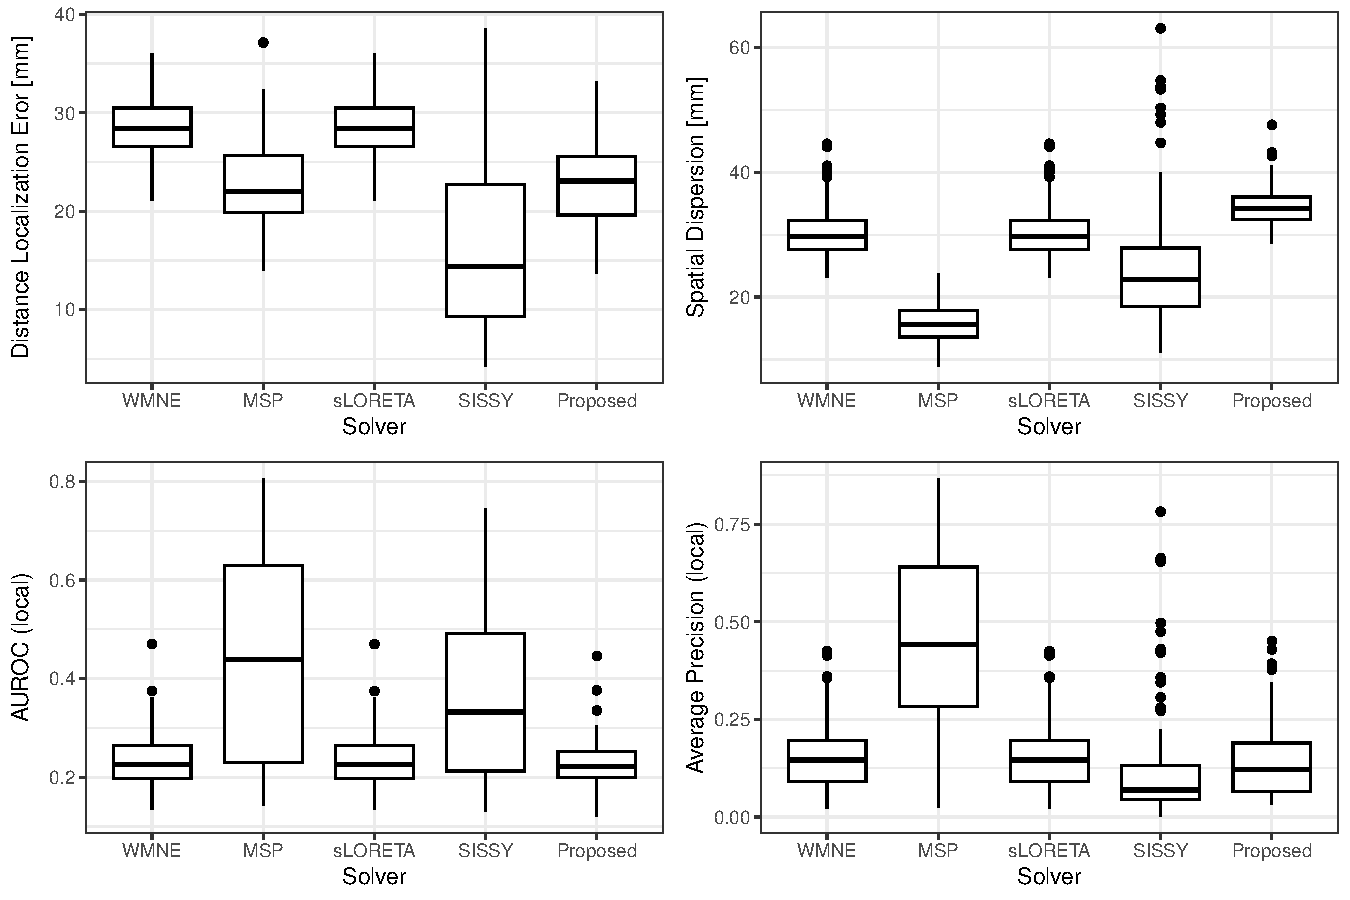
\includegraphics[width=0.9\linewidth]{img_stats/P_plot_EvalMetrics_Protocol04_30ALL.pdf}
    \caption{Performance metrics for some linear estimators, including the proposed one, for the Human synthetic dataset. The dataset contains 30 trials per shape of source patch, and SNR is set to 30 dB}
    \label{fig:results1_P}
\end{figure}

\begin{table}[]
\centering
\begin{tabular}{@{}lllll@{}}
\toprule
      & SD    & AUROC & AP    & Depth  \\
\midrule
DLE   & 0.733 & -0.477 & -0.054 & -0.097 \\
SD    &       & -0.555 & -0.393 & 0.079  \\
AUROC &       &        & 0.536  & -0.103 \\
AP    &       &        &        & -0.108 \\
\bottomrule
\end{tabular}
\caption{Pearson correlation between performance metrics for the proposed estimator and the Human dataset.}
\label{tab:corr_P}
\end{table}

\begin{figure}
    \centering
    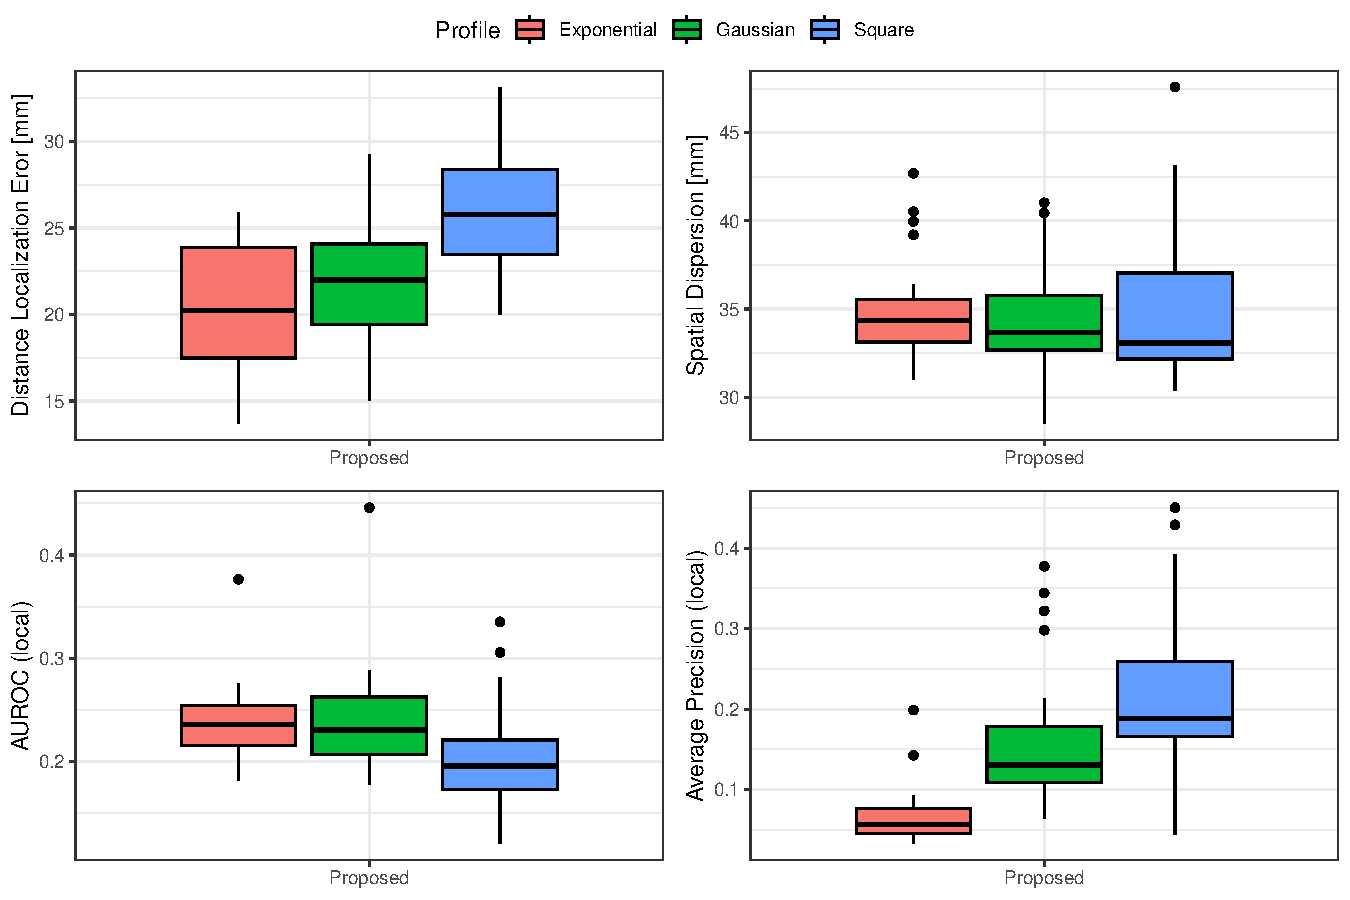
\includegraphics[width=0.9\linewidth]{img_stats/P_shape_EvalMetrics_Protocol04_30ALL.pdf}
    \caption{Changes in performance metrics for the proposed estimator with the Human dataset when different shapes of source patches are used.}
    \label{fig:deets_P}
\end{figure}

\begin{figure}
    \centering
    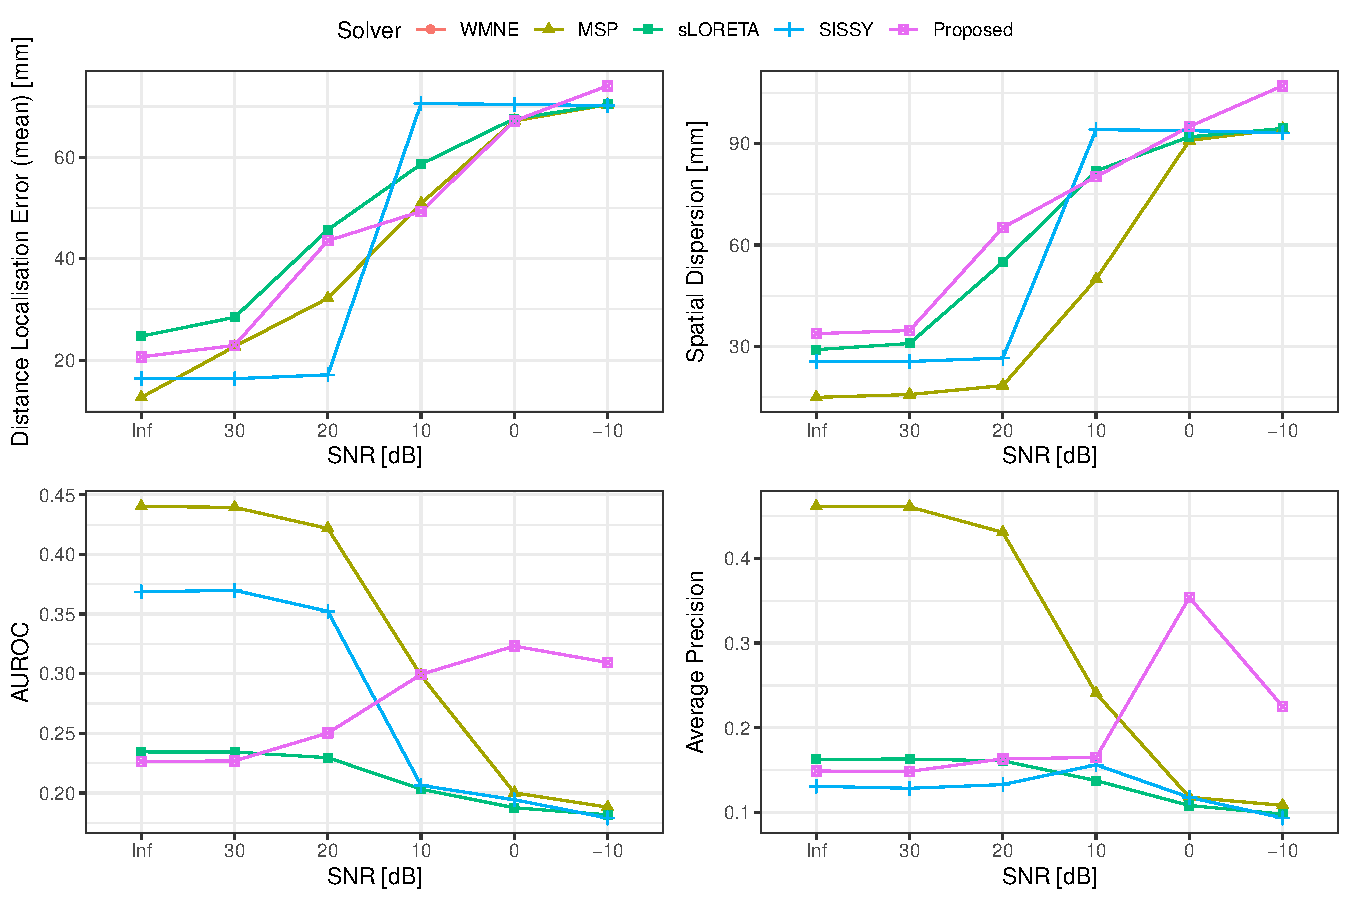
\includegraphics[width=0.9\linewidth]{img_stats/P_SNRdegradation_EvalMetrics_Protocol04_30.pdf}
    \caption{Changes in performance metrics for the proposed estimator with the Human dataset as the as the SNR decreases}
    \label{fig:noise_degradation_P}
\end{figure}

The results from these numerical experiments are collected in the
figures \ref{fig:results1_P}, \ref{fig:deets_P}, and \ref{fig:noise_degradation_P}, as well as in table \ref{tab:corr_P}.
%
These figures are extensions of figures
\ref{fig:results1}, \ref{fig:deets_SISSY}, and \ref{fig:noise_degradation} with additional data.
%including data using the proposed solver.
%
%This allows for a quick comparison.
%
The findings from these observations may be summarised as follows:
\begin{itemize}
    \item The proposed solver outperforms the linear methods in Distance Localization Error but is outperformed by them in Spatial Dispersion.
    \item The proposed method is quite sensible to the shape of the source patch. 
    \item The proposed method seems to outperform all methods, including SISSY, in high-noise conditions, as seen by AUROC and Average Precision.
    \item For the proposed method, performance degradation due to increasing noise is unremarkable --when compared with other linear estimators.
\end{itemize}

Source patches that resemble point sources, such as the exponential profile, are more easily recovered by all methods; the proposed method is no exception.
%
Average Precision seems to be particularly sensible to the labels created using different shapes of source patches.

The presence of P-regions can explain the proposed method's high performance in the classification metrics: the location of the source is already given, to some extent, independently of noise.
%
In other words, the additional information gives a hot start in creating estimated labels.

The proposed method's advantages seem marginal; they stay within the expected values for linear estimators.

\subsection{Synthetic Data (Animal Model)}

%The effectiveness of the proposed ESI method is tested using synthetic data.
%
%The protocol used to create this set of trials is similar to that of Chapter \ref{ch:numeric}, but using the anatomy of an animal model.
%
%This is done in preparation for the analysis of real data.

\subsubsection{Forward Model}

We consider a young male from the species \textit{Sus scrofa}: Yucatan minipig for this synthetic dataset.
%
This selection follows from the real data used in the next subsection in preparation for it.

Anatomical data was obtained from an age-matched publicly available MRI template published by Joanne et al. \cite{pig_template}.

The skull-stripped MRI was segmented using 
%the Freesurfer software; the specific methods used can be traced to the paper by Segone et al. \cite{spf2007}.
the CAT12 software \cite{gaser2022cat}.
%
We used the provided skull-tripped MRI to accommodate the anatomical differences concerning human subjects.
%
Later, the cortex surface and its envelope were reconstructed; both surfaces are displayed in figure \ref{fig:surfaces_pig}.

\begin{figure}
\centering
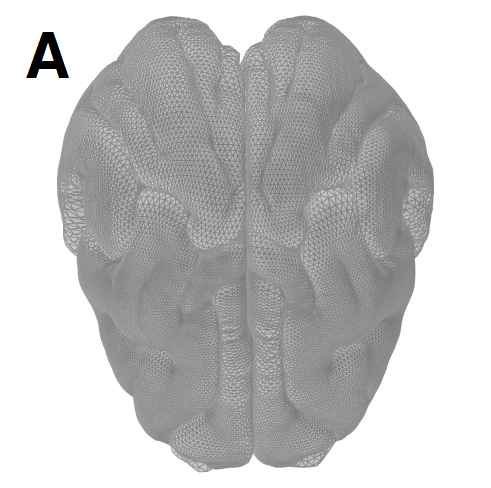
\includegraphics[width=0.18\linewidth]{./img_dev2/3D_subject17_top}
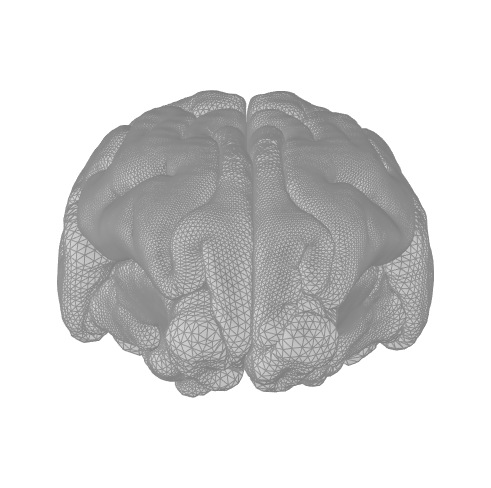
\includegraphics[width=0.18\linewidth]{./img_dev2/3D_subject17_front}
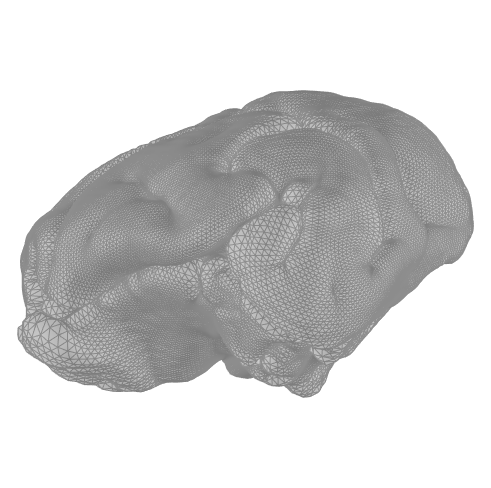
\includegraphics[width=0.18\linewidth]{./img_dev2/3D_subject17_left}
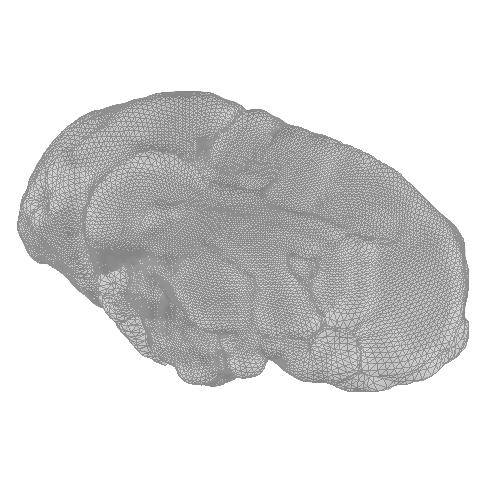
\includegraphics[width=0.18\linewidth]{./img_dev2/3D_subject17_left_in}
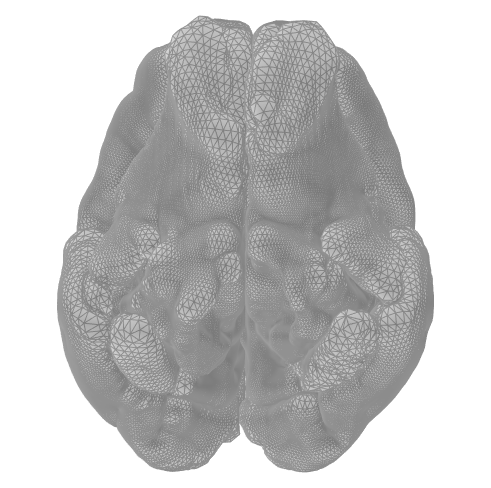
\includegraphics[width=0.18\linewidth]{./img_dev2/3D_subject17_bottom}
%
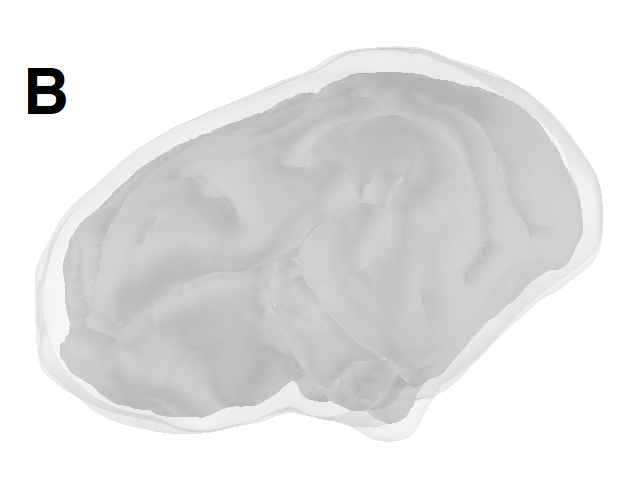
\includegraphics[width=0.23\linewidth]{./img_dev2/3D_subject17_compositeA}
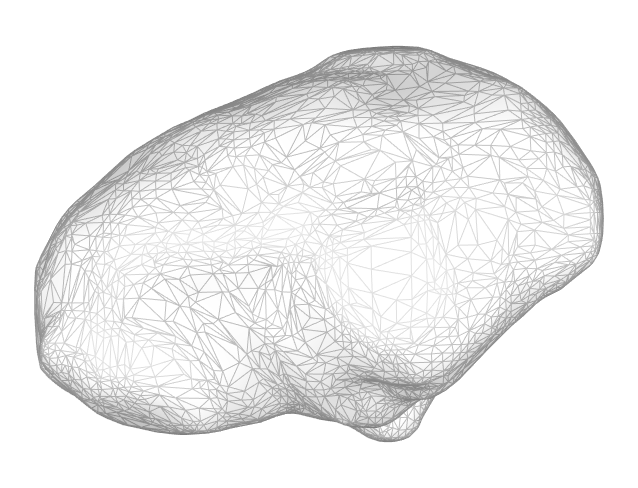
\includegraphics[width=0.23\linewidth]{./img_dev2/3D_subject17_compositeB}
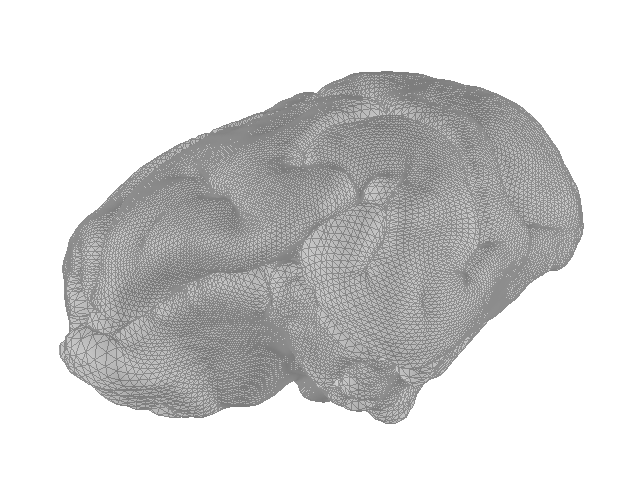
\includegraphics[width=0.23\linewidth]{./img_dev2/3D_subject17_compositeC}
\caption{A. Cortex surface for the \textit{Sus scrofa} template by Joanne et al. \cite{pig_template}, consisting of 8,395 vertices. Views from top, front, left, right, bottom. B. Triangulated surfaces used for the 2-sphere forward model: cortex, cortex envelope}
\label{fig:surfaces_pig}
\end{figure}

Following the protocol from the real data, a total of 8 surface electrodes were placed at the cortex; the placement is 10 mm parallel to the Central Line and 10 mm away from the Anterior Edge.
%
See figure \ref{fig:pig_elecs} for a visual guide of the locations of the electrodes.

\begin{figure}
\centering
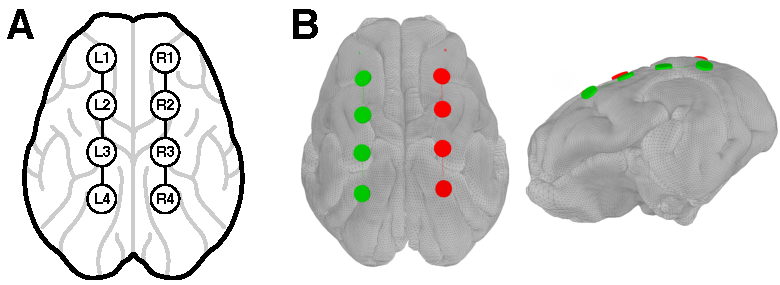
\includegraphics{./img/electrodes_pig.pdf}
\caption{A. Approximate location and labels for the surface electrodes on a diagram. B. Electrode locations on the cortex triangulated surface}
\label{fig:pig_elecs}
\end{figure}

An adaptive layer of $N=4,940$ unconstrained dipole sources was constructed over the brain volume.
%
For the forward model, we considered only the surface ECoG electrodes ($M=8$).
%
Only one single point in time was considered ($T=1$).

For this particular model, a 2-sphere model was constructed with the media being (1) the brain and (2) the space between the cortex and its envelope.
%
This second media is justified because the CSF and connective tissues were not removed from the subject; additionally, it is required computationally due to the reflective conditions at the outer layer.
%
See chapter \ref{ch:forward} for more details.

The leadfield matrix was computed using OpenMEEG \cite{gramfort2010openmeeg} within the Brainstorm toolbox \cite{brainstorm}.

\subsubsection{Results}

As for the previous synthetic dataset, the proposed method is tested.
%
A single P-region is constructed per each trial, following the same protocol with $\kappa =$ 8.95 mm.
%
This value of $\kappa$ was selected so that the resulting source patches have an approximate volume of 3 $\text{cm}^3$, which is similar to the volume of the region with pathological symptoms observed in the real data.

The battery of visualizations from figures \ref{fig:results1_pig}, \ref{fig:deets_pig}, and \ref{fig:noise_degradation_pig} tell us similar information as with the other synthetic dataset: the performance of the proposed method is within the expected, and the estimation is affected by the shape of the source patches.

As for the other datasets, in table \ref{tab:corr_pig}, we have confirmation that the Distance Localization Error and the Spatial Dispersion are correlated, as well as AUROC and Average Precision.
%
None of the variables is significantly correlated with the depth of the source patch.

For this particular dataset, the performance degradation due to increased noise is not very aggressive.
%
This can be explained by the smaller brain volume, which makes the source patches relatively bigger.

\begin{figure}
    \centering
    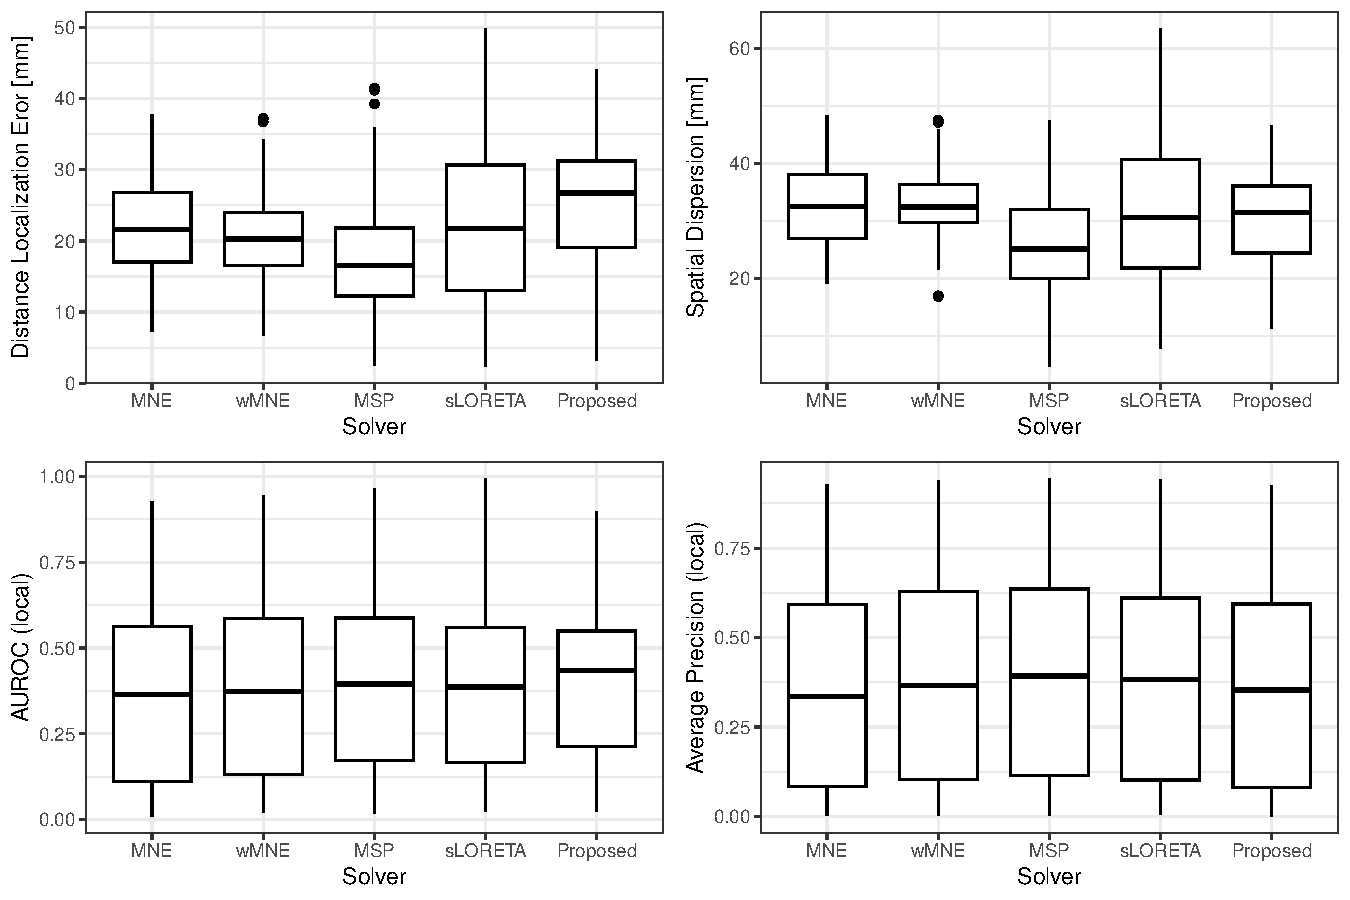
\includegraphics[width=0.9\linewidth]{img_stats/pig_plot_EvalMetrics_protocol04_vol5k_pigALL.pdf}
    \caption{Performance metrics for some linear estimators, including the proposed one, for the Animal Model synthetic dataset. The dataset contains 100 trials per shape of source patch, and the SNR is set to 20 dB}
    \label{fig:results1_pig}
\end{figure}

\begin{table}[]
\centering
\begin{tabular}{@{}lllll@{}}
\toprule
      & SD    & AUROC & AP    & Depth  \\
\midrule
DLE   & 0.870 & 0.138 & 0.105 & -0.192 \\
SD    &       & 0.028 & 0.008 & -0.144 \\
AUROC &       &       & 0.957 & -0.035 \\
AP    &       &       &       & -0.063 \\
\bottomrule
\end{tabular}
\caption{Pearson correlation between performance metrics for the proposed estimator and the Animal Model dataset.}
\label{tab:corr_pig}
\end{table}

\begin{figure}
    \centering
    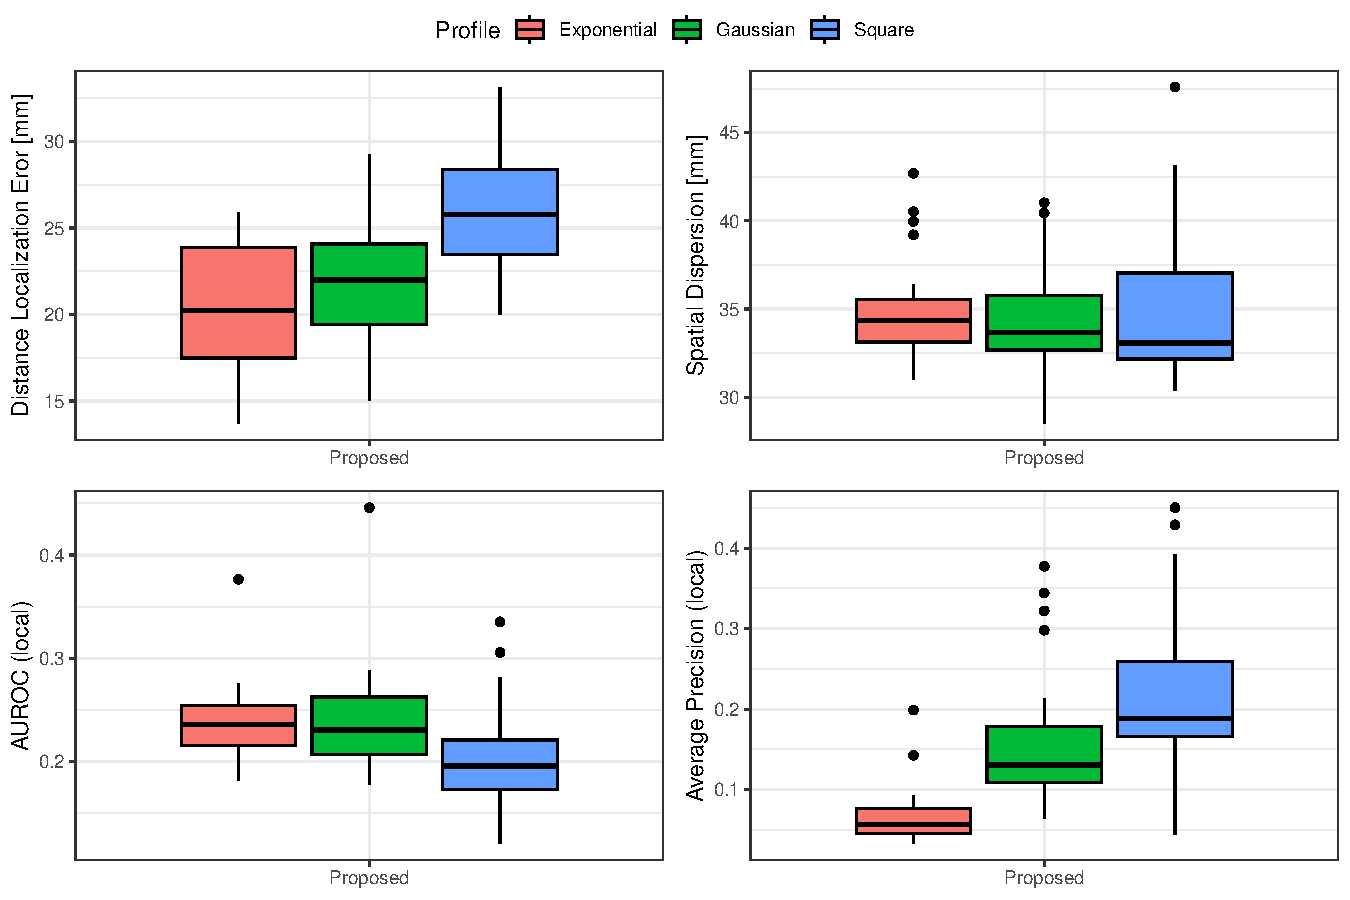
\includegraphics[width=0.9\linewidth]{img_stats/P_shape_EvalMetrics_Protocol04_30ALL.pdf}    
    \caption{Changes in performance metrics for the proposed estimator with the Animal Model dataset when different shapes of source patch are used}
    \label{fig:deets_pig}
\end{figure}

\begin{figure}
    \centering
    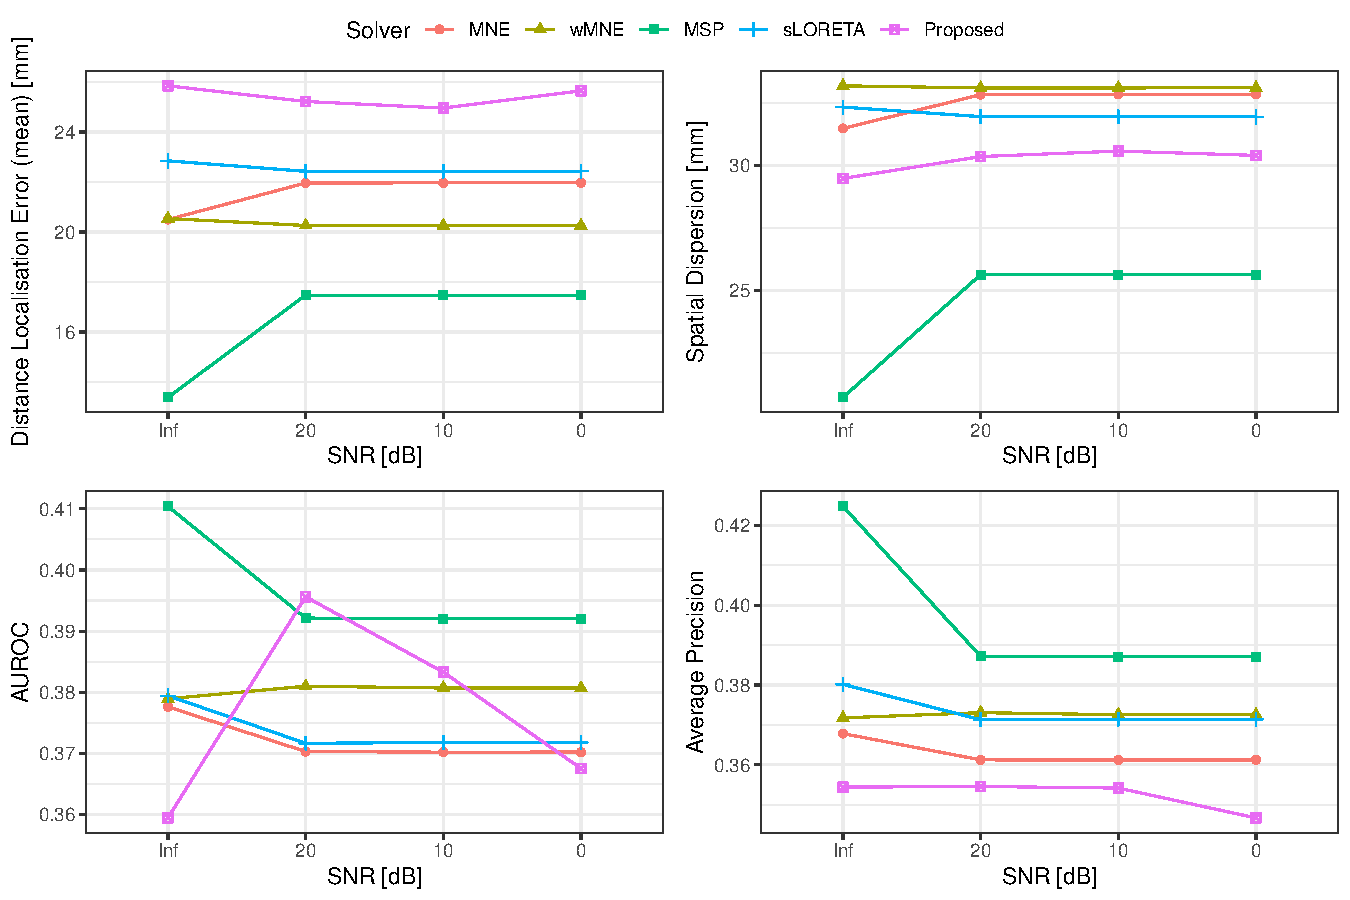
\includegraphics[width=0.9\linewidth]{img_stats/pig_SNRdegradation_EvalMetrics_protocol04_vol5k_pig.pdf}
    \caption{Changes in performance metrics for the proposed estimator with the Animal Model dataset as the SNR decreases}
    \label{fig:noise_degradation_pig}
\end{figure}

\subsection{Real Data}
\label{sec:real_data}

The effectiveness of the ESI method is tested using data from an experiment of acute ischemic stroke on an animal model performed by Dr. J. Pascal et al. at UT Southwestern Medical Center \cite{pig_lesion1, PMID_36109613}.

Acute Ischemic Stroke was induced in the subject by obstruction of the Middle Cerebral Artery.
%
In summary, a stroke is the obstruction of a vein or artery in the brain, which stops the supply of oxygenated blood.
%
The brain regions affected by hypoxia (lack of oxygen at a cellular level) are called the Ischemic Penumbra.

This procedure is referred to as the induced lesion for ease of notation.

\subsection{Pathology Data}

Posterior to the experiment, the subject was sacrificed.
%
During a post-mortem analysis, the subject's brain was extracted and sliced in order to be stained with 
2, 3, 5 triphenyltetrazolium (TTC).

The operation of the TTC staining is based on the fact that TTC (white) 
%is a white compound, but it 
is degraded to 1,3,5-triphenyl formazan (TPF, red)
on the presence of dehydrogenases in metabolically active cells.
%
As a result, tissue colored white was affected by necrosis, and tissue colored red was unaffected \cite{li2018use}. 

\begin{figure}
\centering
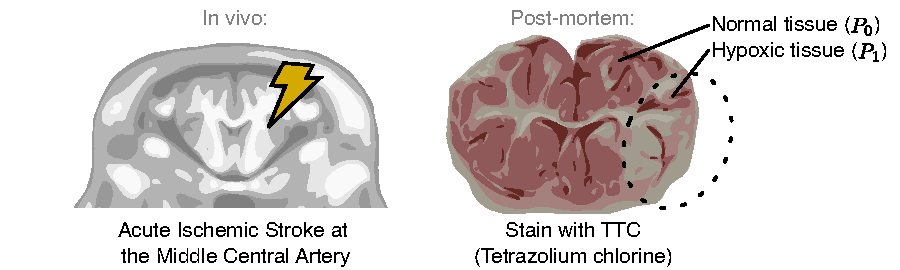
\includegraphics[width=\linewidth]{./img/Pregions_real.pdf}
\caption{P-regions are determined based on observed symptoms from a pathology: the TTC stain colors normal tissue as white and hypoxic tissue as red.
%
Hypoxia is due to an induced acute ischemic stroke in the Middle Cerebral Artery on an animal model (pig)
%
%Although the stroke occurred in vivo with ECoG monitoring, the TTC stain is only possible post-mortem
}
\label{fig:Preg_real}
\end{figure}

Within the framework of this work, pictures obtained after TTC staining were registered to the template MRI to identify retroactively the Ischemic Penumbra at the time of the ECoG recordings.
%
%This definition is simplistic and doesn't represent a clinical decision.

With this information, we constructed the P-region $P_1$ as the Ischemic Penumbra and the rest of the brain as the region $P_0$.
%
See figure \ref{fig:Preg_real} for a guide to this process.
%
%The selection of one single P-region follows the observed data.
%
Although the model can consider multiple P-regions, based on the observed data, only one region is used for this dataset.

\subsection{Results}

After using the TCC data to construct the P-regions, the proposed method was used over recordings from the subject after the induced lesion.
%
Other ESI methods (wMNE, MSP, and sLORETA) were also tested on the same dataset for comparison.

Here, we show an image from the reconstruction at $t=78.507$ s after the lesion was performed.
%
As shown in figure \ref{fig:real_ecog}, a small peak can observed at this point in time.
%
However, this specific point in time is not of particular interest; it is merely presented as an example to compare the behaviors of different ESI methods.

\begin{figure}
\centering
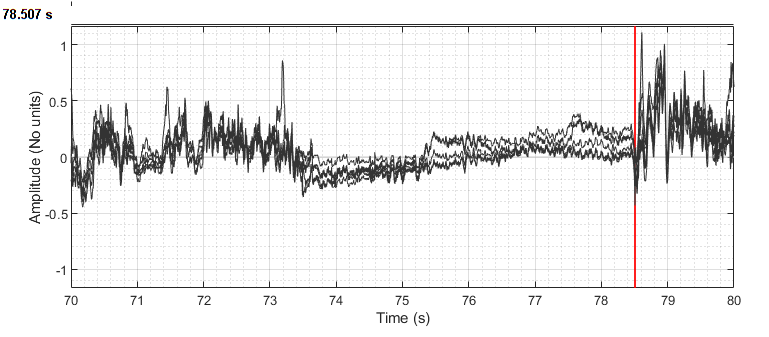
\includegraphics[width=0.9\linewidth]{./img_dev2/ECOG_All_sub17diss_diss1}
\caption{Recordings from surface electrodes. The point in time used for figure \ref{fig:real_comp} is highlighted.
Time is measured after the induced lesion}
\label{fig:real_ecog}
\end{figure}

\begin{figure}
\centering
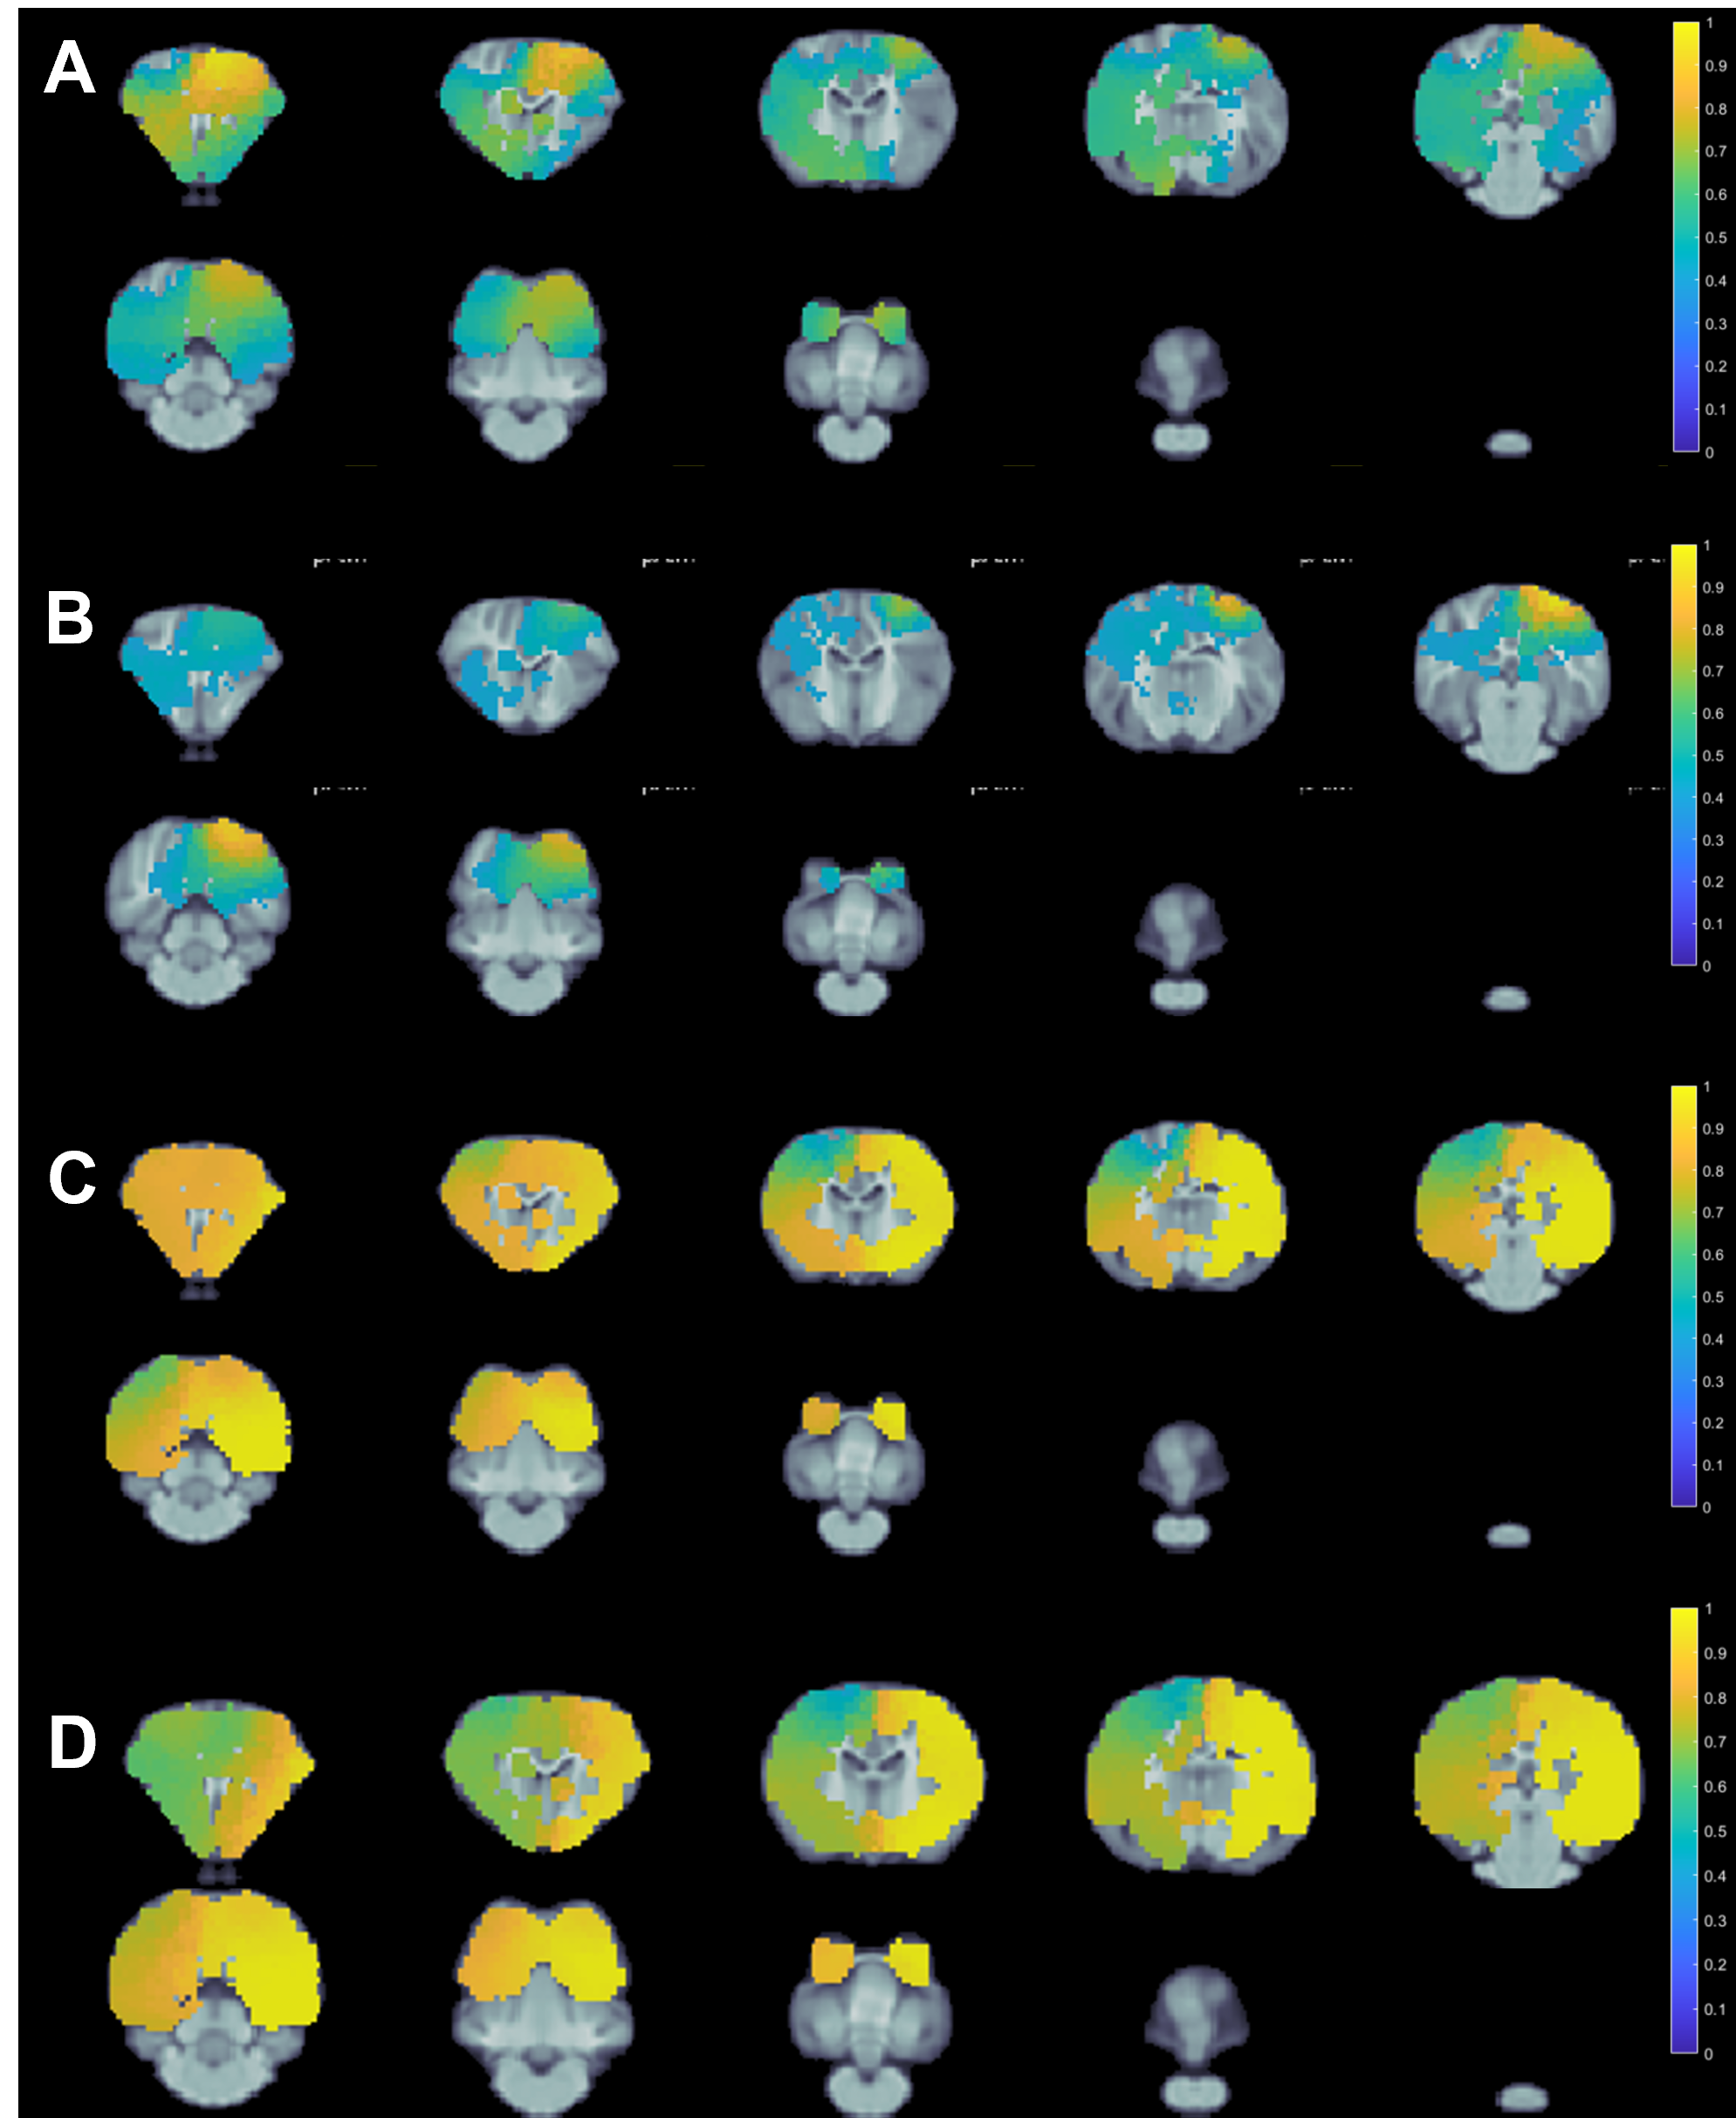
\includegraphics[width=0.9\linewidth]{./img_dev2/real_comparison}
\caption{Coronal slices of the subject's brain displaying the magnitude of distributed dipoles; maximum magnitude was scaled to 1 for comparison.
%
Results were obtained using various ESI methods: wMNE (A), MSP (B), sLORETA (C), and the proposed method (D)}
\label{fig:real_comp}
\end{figure}

In figure \ref{fig:real_comp}, we can observe the cortical activations: the estimated magnitudes of the distributed dipoles superimposed with the subject's MRI.
% 
A few coronal slices were used to illustrate the 3D extent of the estimations.

Notice that wMNE and MSP suffer from depth weighting as their estimations are concentrated near the cortex, especially near the sensors.
%
These estimations are also relatively compact in space, which is a positive quality.

On the other hand, sLORETA is spread throughout the whole volume, making it difficult to judge whether it is sensible to the depth of the sources.

The proposed method behaves much like sLORETA.
%
Although the spread is similar, we can observe a slightly better focus in space, with regions far from the source possessing lower magnitudes.
%
Notice that the high amplitude region is diffusively aligned with the P-region shown in figure \ref{fig:Preg_real}.

The numerical experiments show that source localization is not heavily correlated with depth for one simple case: a single source patch of relatively small size.
%
We observed that all ESI methods under consideration, including the proposed method, reconstruct better sources whose shape is similar to a point source.

The results from real data suggest that the real source patch may be large in size, and its shape is not similar to a point source.

Based on this data, we can infer that wMNE and MSP enforce the minimal-norm assumption by preferring point-like solutions. In contrast, the sLORETA assumption of smoothness in space is more appropriate for large sources but leads to overspreading.
%
The proposed method's additional information makes it prefer sources located near or at $P_1$, but it also selects sources that extend on the entirety of $P_1$ and beyond.

For future work, we suggest using this assumption in combination with stronger assumptions of minimal-norm. 
%
Maybe the concept of P-regions can be combined with methods based on the $\ell_1$ norm.